% =====================================================================
%  MIG 2026 SHORT PAPER  (4-6 pages EXCLUDING references, per the CFP)
%
%  Builds with:  latexmk -pdf main_short.tex
%
%  This is FRESH CONDENSED TEXT, not a fork of sections/*.tex (per
%  ../docs/mig2026_short_paper_plan.md 3). The long paper stays main.tex.
%
%  EVERY NUMBER HERE IS FROZEN IN ../docs/mig2026_results_ledger.md with its
%  generating command, commit and machine. Do not edit a number here without
%  editing it there.
%
%  BINDING CLAIM DISCIPLINE (plan 1 + the two addenda in
%  ../docs/novelty_positioning.md). Never claim, anywhere in this file:
%   - the contact row / gap / deformed contact point as ours (it is a
%     transcription of the Zheng-James velocity-level law);
%   - two-way coupling, momentum consistency, or "first modal DOFs in XPBD"
%     (write "as contact DOFs" if the point must be made at all);
%   - the under-convergence-injection OBSERVATION (Wei et al. 2026 states it
%     plainly -- cite them for it);
%   - "makes it trustworthy" (write "satisfies a prescribed cumulative
%     modal-storage bound");
%   - unqualified "real-time";
%   - the acronym "DCR" (cite Coevoet et al. or "the one-way baseline").
%  The 1e5 figure is ALWAYS defined as peak modal energy / incident rigid
%  kinetic energy, in adversarial low-budget cells, never production settings.
%  The invariant is ALWAYS written cumulatively, never per-step.
% =====================================================================
\PassOptionsToPackage{dvipsnames,table}{xcolor}
\documentclass[sigconf,screen,review,anonymous]{acmart}

\setcopyright{none}
\acmConference[MIG '26]{The 19th ACM SIGGRAPH Conference on Motion,
  Interaction and Games}{December 11--13, 2026}{Charleston, SC, USA}
\acmBooktitle{The 19th ACM SIGGRAPH Conference on Motion, Interaction and
  Games (MIG '26), December 11--13, 2026, Charleston, SC, USA}
\acmDOI{}
\acmISBN{}
% Placeholder: EasyChair assigns this at registration (window opens 2026-07-25).
% Fill before submission; leaving it empty is harmless in review mode.
\acmSubmissionID{}

\usepackage{pifont}
\graphicspath{{figures/}}
\setlength{\emergencystretch}{8pt}

\newcommand{\dErig}{\Delta E_{\mathrm{rig}}}
\newcommand{\Emod}{E_{\mathrm{mod}}}
\newcommand{\todo}[1]{\textcolor{red}{\textbf{[TODO: #1]}}}

\begin{document}

\title{When Modal Contact Rows Fail in Fixed-Budget XPBD:\\
  Diagnosis and an Operating Guide}

\author{Anonymous Author(s)}

\begin{abstract}
Rigid-body XPBD engines already resolve contacts and joints, and a small global
modal state ($16$--$24$ amplitudes) is an attractive way to give a stiff prop
low-cost vibration without converting it into a full nodal or tetrahedral
deformable. We show that inserting this globally shared modal state directly
into a two-way unilateral contact row is not automatically energy-safe when the
host runs only a few local iterations per substep. Across three scenes, two
relaxations, and four schedules, our tested XPBD implementation overdraws the
measured gross rigid-side supply by up to $4.4\times10^{7}$~J (a
$2.2$--$4.5\times10^{7}$~J neighborhood over a deterministic perturbation
ensemble), whereas augmented-Lagrangian and implicit implementations are
markedly milder controls: at most $6.7$~J in $3$ of $24$ cells, and never,
respectively (an accounting audit places the control floor below $10^{-3}$~J, so
the $6.7$~J is real injection). An iteration ladder, equal-row-count schedules,
warm starting, mode truncation, and a block-condensation ablation localize the
amplification to finite-budget convergence of the shared modal coupling. When
the contact architecture is flexible, the tested stiffness-aware implicit
realization is the preferred observed control; in a fixed XPBD host the budget
is best spent on iterations, with a verified basis, since more substeps and a
block solve do not suffice. For hosts
that still cannot converge the row, a cumulative modal-storage projection
enforces its accounting bound unconditionally (Prop.~\ref{prop:guarantee},
roundoff floor in all $90$ measured cells). Since the bound fixes only where the
projected state lands, that projection can be chosen to hold the
contact-observed surface fixed, cutting the penetration it opens from
$2.4$--$47.6\times$ the truncated solve's own to $1.0$--$6.3\times$: the
residual is the price of the un-converged row, not of the guardrail, and this is
containment rather than corrected contact.
\end{abstract}

\begin{CCSXML}
<ccs2012>
<concept><concept_id>10010147.10010371.10010352.10010379</concept_id>
<concept_desc>Computing methodologies~Physical simulation</concept_desc>
<concept_significance>500</concept_significance></concept>
</ccs2012>
\end{CCSXML}
\ccsdesc[500]{Computing methodologies~Physical simulation}
\keywords{contact, modal reduction, position-based dynamics, energy safety,
  fixed-budget solvers}

\maketitle

\begin{figure}[t]
\centering
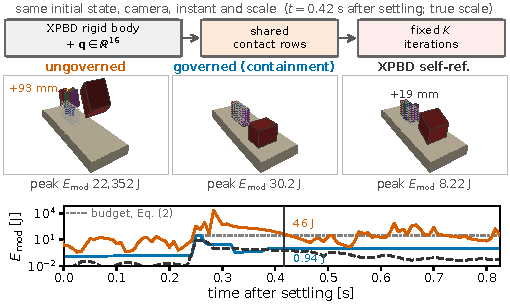
\includegraphics[width=\columnwidth]{fig_teaser.pdf}
\caption{One shelf impact at a production-like interactive budget
($1{\times}8$), true scale, three independent runs. Ungoverned, truncation
energy throws the resting books up to $93$~mm, more than their own height.
Governed, \eqref{eq:invariant} holds peak modal energy to $29.5$~J and they stay
within $1$~mm of rest; the reference is the host's own high-iteration run
($500{\times}1$). The bound removes the spurious launch and some legitimate
motion with it: the reference lifts one book $19$~mm, the governed run none.}
\label{fig:teaser}
\end{figure}

% =====================================================================
\section{Introduction}
% =====================================================================
A developer building an interactive scene on a rigid-body XPBD
engine~\citep{macklin2016xpbd} already has a solver that resolves contacts and
joints under a small, fixed local-iteration budget. To make a stiff prop such
as a shelf, a table, or a ledge ring when it is struck, one option is to
replace it with a full nodal or tetrahedral deformable, at the cost of
thousands of online coordinates and local internal constraints; the lighter
alternative is to attach a small precomputed modal basis, $16$--$24$ global
amplitudes $\mathbf{q}$ that capture
the low-frequency bending of a stiff, small-displacement
body~\citep{james2002dyrt,hauser2003,peng2024reduced}. The runtime state grows
by a handful of numbers, the precomputation is offline, and the same XPBD host
steps everything. This paper is written for that developer; it does not argue
XPBD against another solver.

The difficulty lies in the contact. In the real-time precedent the modal prop
is driven \emph{one way}: an external filter reads detected contact events and
rings the modes with no back-reaction~\citep{coevoet2020distant}. This
double-counts the interface energy and cannot let the prop's own deformation
change how it is supported. The physically consistent alternative is a
\emph{two-way} row, in which rigid and modal unknowns are resolved together
through one shared contact multiplier~\citep{zheng2011}, so that a heavier load
bends the support and the bent support redistributes the load. The risk is that
every support contact touches the same global vector $\mathbf{q}$: the
contact-row graph is dense on the modes even though the state is small, and a
host running only a few local iterations per substep need not converge that
shared coupling. We take the row as given: at position level it is one
linearization step from the velocity-level law
($C^{n+1}\!\approx\!C^{n}+h\,\mathbf{J}\mathbf{u}^{n+1}$, same Jacobian and
multiplier as~\citet{zheng2011}), it is narrower than the original (normal rows
only, $e{=}0$ restitution), and it is not a contribution of this paper. Our
question is the practitioner's: what does the direct two-way transcription cost
at a normal budget, and what should one do about it? Where solver architecture
is unconstrained, our evidence favors the tested stiffness-aware velocity-level
realization; our target, however, is the existing fixed-budget XPBD host.

Finite-iteration coupling across a partition boundary can inject spurious energy
even when every subsystem is individually passive~\citep{wei2026earlyterm}, and
velocity-level frictional contact spanning rigid and reduced deformable bodies,
with the energy artifacts of iterative solvers named, goes back at least
to~\citet{kaufman2008}. What has been missing is a quantitative account of the
present case (unilateral contact-to-modal transfer in a fixed-budget host) and
an operating guide for the practitioner who encounters it; this paper supplies
both.

\paragraph*{Contributions.}
\begin{enumerate}
\item \textbf{A practitioner workflow and its failure.} We treat adding a compact
  modal state to a fixed-budget XPBD host as the workflow it is, and show that the
  direct two-way contact row overdraws its measured rigid-side supply
  catastrophically at interactive budgets, across three scenes, two relaxations,
  and four schedules (\S\ref{sec:matrix}), with augmented-Lagrangian and
  implicit implementations as milder controls. The cross-control reading is
  supported by a gravity/no-contact accounting audit, and the robustness of the
  failure by a deterministic perturbation ensemble.
\item \textbf{Mechanism and an operating guide.} A same-path iteration ladder,
  equal-row-count schedules, warm starting, mode truncation, and an in-host
  block-condensation ablation localize the amplification to finite-budget
  convergence of the shared modal coupling (\S\ref{sec:kconv}), and yield an
  ordered decision rule: the tested implicit realization when the architecture is
  flexible; otherwise, in a fixed XPBD host, iterations and a verified basis
  rather than more substeps or a block solve.
\item \textbf{A last-resort guardrail and its price.} A cumulative modal-storage
  bound funded by the measured rigid-side loss and enforced by a scalar
  projection of the realized state (\S\ref{sec:bound}). It is a deliberately
  minimal fail-safe rather than a contact method: guaranteed unconditionally
  (Prop.~\ref{prop:guarantee}, roundoff floor in all $90$ measured cells), but
  at a measured cost to contact validity (\S\ref{sec:validity}).
\end{enumerate}

\paragraph*{Related work.} Rigid XPBD~\citep{macklin2016xpbd}, interactive modal
deformation and velocity-level modal contact~\citep{james2002dyrt,hauser2003,%
zheng2011,kaufman2008}, and reduced XPBD~\citep{peng2024reduced} set the stage;
the last uses modes as a deformation surrogate, whereas here modal
amplitudes enter as contact DOFs driven by the shared multiplier
(cf.~ray-traced penalty contact without a shared unilateral
multiplier~\citep{zobel2025unity}). Our last-resort guardrail adapts
energy-tank control~\citep{hannaford2002,franken2011,rath2008} rather than
inventing a new mechanism: we keep the tank-and-observer structure, but we fund
the tank from the measured rigid-side loss rather than from the port it
regulates, and we scale the realized state rather than a force, because a
fixed-budget solver commits its multipliers before the excess is observable.
These choices separate it from total-energy projection~\citep{dinev2018fepr},
bidirectional total-energy tracking~\citep{you2026energy}, and the structural
finite-budget passivity of bilateral couplings~\citep{wei2026earlyterm}.

% =====================================================================
\section{The row and the invariant it must respect}
\label{sec:row}
% =====================================================================
Let $\mathbf{q}\in\mathbb{R}^{r}$ be mass-normalized modal amplitudes of the
supporting body, so its modal mechanical energy is
$\Emod=\tfrac12\dot{\mathbf{q}}^{\!\top}\dot{\mathbf{q}}
      +\tfrac12\mathbf{q}^{\!\top}\mathbf{K}\mathbf{q}$.
A support-contact row between a rigid corner at world height $y_c$ and the
deformed surface has gap
\begin{equation}
C \;=\; y_c \;-\; \bigl(y_{\mathrm{rest}} + \mathbf{U}_y^{\!\top}\mathbf{q}\bigr),
\qquad C \ge 0,\; \lambda \ge 0,\; C\lambda = 0,
\label{eq:row}
\end{equation}
with $\partial C/\partial\mathbf{q}=-\mathbf{U}_y$, so one multiplier $\lambda$
drives both the rigid body and the modal amplitudes. Equation~\eqref{eq:row} is
the transcription discussed above, not a new law. It is a single row law,
instantiated at every support contact in every substep ($48$ such rows on the
shelf, $40$ on the ledge, $200$ on the table), with all rows sharing the one
modal state $\mathbf{q}$.

\paragraph*{The invariant.} We require that the energy stored in the modal
subsystem never exceed the measured gross rigid-side loss, defined exactly at
\eqref{eq:derig} below, cumulatively over the run:
\begin{equation}
\Emod^{\,n} - \Emod^{\,0}
\;\;\le\;\;
\eta \sum_{k\le n} \max\!\bigl(\dErig^{\,k},\,0\bigr),
\qquad \eta\in(0,1].
\label{eq:invariant}
\end{equation}
The transfer efficiency $\eta$ sets how much of the measured loss may be spent;
every experiment in this paper runs $\eta=1$, the least restrictive admissible
value, so no result below depends on tuning it. The bound is cumulative rather
than per-step: a substep may deposit more than it earns provided the running
total remains within the budget, which is what allows a legitimate ring to
persist across substeps.

\paragraph*{Definitions.} Modal storage is the mechanical energy of the
reduced state as written above, and $\Emod^{\,0}=0$: every scene starts from an
undeformed, resting support, so even the run's own settling transient must be
funded by the reservoir. The supply is
\begin{equation}
\dErig^{\,k} \;=\; \bigl(E_{\mathrm{rig}}^{k,-} - E_{\mathrm{rig}}^{k,+}\bigr)
                 \;+\; W_g^{\,k},
\qquad
W_g^{\,k}=\sum_b m_b\,\mathbf{g}\!\cdot\!\bigl(\mathbf{x}_b^{k,+}-\mathbf{x}_b^{k,-}\bigr),
\label{eq:derig}
\end{equation}
where $E_{\mathrm{rig}}=\sum_b\bigl[\tfrac12 m_b\|\mathbf{v}_b\|^2
+\tfrac12\boldsymbol{\omega}_b^{\!\top}\mathbf{I}_b\boldsymbol{\omega}_b\bigr]$
is purely kinetic (over all dynamic bodies, not merely those in contact) and
$\pm$ denote the two ends of substep $k$. We call this the \textbf{measured
gross rigid-side loss}. It is a loss, not a dissipation: it also counts
legitimate rigid-to-modal transfer and losses at rigid--rigid contacts elsewhere
in the scene, so it is an envelope on what contact dissipated rather than a
measurement of it (\S\ref{sec:limits}). Gravity enters only through $W_g$, so
free ballistic motion registers zero supply, and only an inelastic velocity
change funds the reservoir. Substep-boundary endpoints tile the timeline
exactly, so no rigid energy change escapes the accounting.

\paragraph*{What the invariant is, and two diagnostics.} The bound
\eqref{eq:invariant} is a cumulative storage ceiling whose supply is measured
rather than prescribed: the right-hand side is the measured loss of
\eqref{eq:derig}, never a tuned constant or a fraction of incident energy. It
constrains a scalar reservoir, not a contact port, so it is neither port
passivity nor a signed per-interface bound. The gross sum ignores substeps in
which the rigid subsystem gains energy, and counts energy returned and
re-dissipated as fresh supply (\S\ref{sec:limits} measures both). We keep two
diagnostics distinct: the incident-energy ratio $R=$~peak modal energy / peak
incident rigid KE, a severity measure, and the signed margin of
\eqref{eq:invariant} in joules, the invariant proper; they need not flag the
same cells. Enforcing the bound requires a projection (\S\ref{sec:bound}).

% =====================================================================
\section{The failure at a fixed budget}
% =====================================================================
All solver-behaviour measurements below come from a single machine (Apple M4,
CPU, CPython 3.12); every number is frozen with its generating command and
commit hash in the supplemental ledger. We deliberately avoid mixing machines,
because chaotic contact stacks diverge across architectures under
floating-point reassociation.

\subsection{One row, three implementations, the same 24 cells}
\label{sec:matrix}

\begin{figure*}[t]
\centering
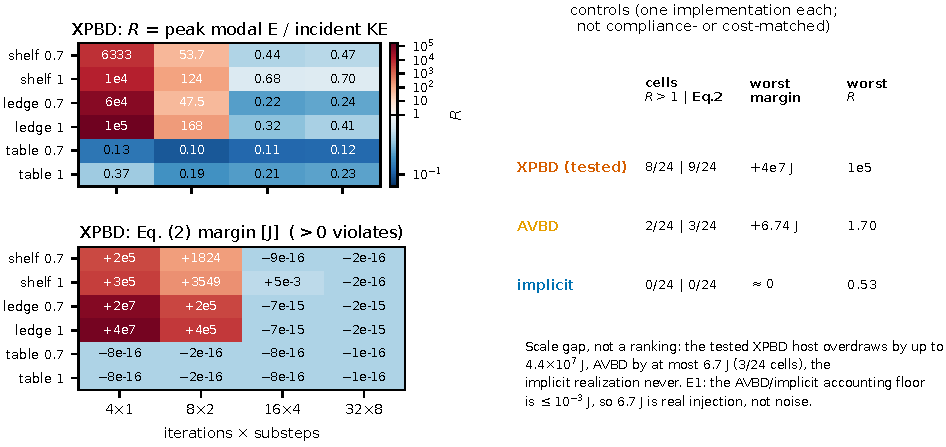
\includegraphics[width=0.70\textwidth]{fig_xpbd_map.pdf}
\caption{Our tested XPBD implementation, over the 24-cell sweep (3 scenes
$\times$ relaxation $\{0.7,1.0\}$ $\times$ budget), governor OFF. \textbf{Left,
top:} $R$ = peak modal energy / peak incident rigid KE, a severity diagnostic;
\textbf{bottom:} the signed margin of \eqref{eq:invariant} in joules ($>0$
violates). The two need not flag the same cells (XPBD: $R{>}1$ in $8/24$,
margin$>0$ in $9/24$); the disagreement is a result, not noise. \textbf{Right:}
a compact control strip for the three implementations (one of each, neither
compliance- nor cost-matched): violating cells, worst margin, worst $R$. The
comparison is a scale gap rather than a ranking: $4.4\times10^{7}$~J vs.\
$\le6.7$~J vs.\ $0$. The accounting audit (supplement E1) puts the control
floor below $10^{-3}$~J, so $6.7$~J is real injection. The full two-metric
72-cell three-implementation heatmap is in the supplement.}
\label{fig:matrix}
\end{figure*}

We drive an impactor into a modally reduced support in three scenes (a shelf
board, a ledge slab, and a $2.2\times1.1$~m table, the last two following the
layouts of \citet{coevoet2020distant}) and sweep modal relaxation and the
local budget (iterations $\times$ substeps) over
$\{4{\times}1, 8{\times}2, 16{\times}4, 32{\times}8\}$. The hosts are
XPBD~\citep{macklin2016xpbd}, AVBD~\citep{giles2025avbd} (a descendant of vertex
block descent~\citep{chen2024vbd}), and a sequential-impulse realization in the
sense of~\citet{catto2005iterative}, made implicit in the modal block. All three
are pinned to $h{=}1/120$~s, per-substep contact regeneration, modal rank
$16/16/24$ (shelf/ledge/table), Rayleigh damping, an implicit-midpoint modal
restoring step, and $\eta{=}1$. They differ in the unknown solved for
(position, position\,+\,multiplier, or velocity), in the modal contact weight
(XPBD's explicit per-mode compliance $1/(H_{ii}h^2{-}1)$ versus the impulse
host's implicit $(\mathbf{M}{+}h\mathbf{D}{+}h^2\mathbf{K})^{-1}$), in warm
start, and in relaxation (the full host/parameter table is in the supplement).
Two differences matter. Relaxation is inert on the impulse host (its implicit
modal weight needs no under-relaxation), so its two relaxation rows are
bit-identical. Warm start also differs ($\lambda\!\leftarrow\!0$ every substep
for the position-based host, carried duals for the others), so the comparison
is as-deployed rather than compliance-matched. Warm start is not the lever,
however: warm-starting the position-based host leaves the footprint unchanged
(the same $8/24$ cells, worst $1.20\times10^{5}$) and is worse at $4{\times}1$
($3.1\times$), since a warm multiplier cannot converge the shared modal DOF
that only iterations converge (\S\ref{sec:kconv}).

\paragraph*{Equal row evaluations, unequal outcome.} A cell costs $K\!\cdot\!S$
row evaluations per frame, so the budget axis spans $\times64$ and conflates two
refinements that are neither interchangeable nor equally costly (a substep also
repeats contact generation and integration). At $32$ row evaluations on the
shelf drop, spent as iterations ($K{=}32,S{=}1$) the ratio is $0.300$ and
\eqref{eq:invariant} holds; spent as substeps ($K{=}4,S{=}8$) the ratio is
$3.13$, overdrawing by $481$~J. Substep refinement alone does not converge the
row.

Figure~\ref{fig:matrix} shows the outcome. The position-based host exceeds
$R=1$ in $8$ of $24$ cells, worst case $1.19534\times10^{5}$ (ledge, relaxation
$1.0$, $4{\times}1$: peak modal energy $4.44\times10^{7}$~J against an incident
$371$~J); the augmented-Lagrangian host does so in $2$ of $24$, both at the
starved $4{\times}1$ corner of the table scene with worst case $1.70$, so it is
not unconditionally benign either. The ordering is scene-dependent and can
invert: taking the worst over scenes at $4{\times}1$, the position-based host is
five orders of magnitude more energetic in the ratio $R$ ($1.2\times10^{5}$ vs
$1.70$), yet on the table scene itself the augmented-Lagrangian host is the
worse ($1.18$ and $1.70$ against a position-based worst of $0.37$). Neither
host dominates across scenes.

\paragraph*{The ratio is not the invariant.} We also measure
\eqref{eq:invariant} directly on all three hosts, ungoverned, running the
reservoir accounting live while forcing $\gamma\equiv1$: every state write in the
enforcement path is guarded by $\gamma<1$, so the trajectory is bit-identical to
an ungoverned run (the ratios above reproduce the independent sweep exactly).
The two diagnostics do not flag the same cells: the position-based host violates
\eqref{eq:invariant} in $9$ of $24$ against $R>1$ in $8$, the
augmented-Lagrangian host in $3$ against $2$, and the implicit host in neither
($0/24$, worst margin at the roundoff floor), so neither diagnostic subsumes the
other. What orders the failures is magnitude: the position-based overdraw
reaches $4.4\times10^{7}$~J, seven orders beyond the largest
augmented-Lagrangian one ($6.7$~J, at the starved $4{\times}1$ table corner) and
beyond the implicit host's exact zero. A gravity/no-contact accounting audit
puts that control floor below $10^{-3}$~J on both non-injecting hosts, so the
augmented-Lagrangian overdraft is real impact-driven injection rather than
accounting noise: three regimes that the ratio diagnostic compresses into one
number.

\subsection{The position-based amplification is a truncation artifact}
\label{sec:kconv}

\begin{figure*}[t]
\centering
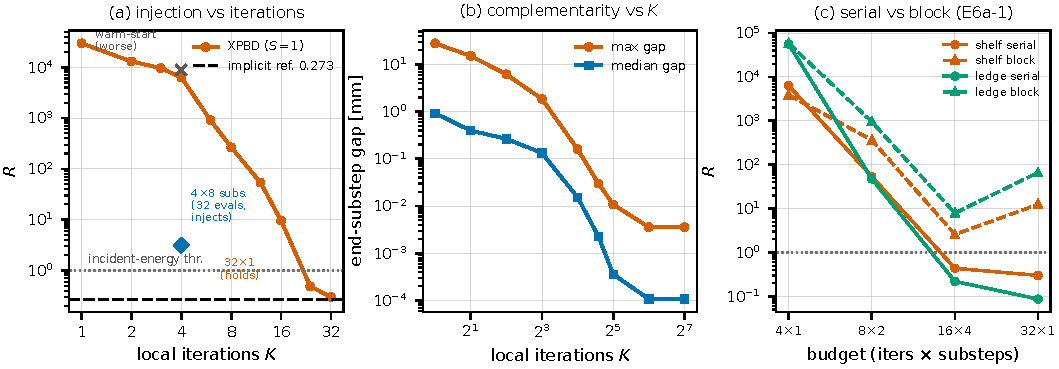
\includegraphics[width=0.76\textwidth]{fig_operating_envelope.pdf}
\caption{The XPBD operating envelope (our tested position-based host, governor
OFF). \textbf{(a)}~Injection $R$ vs.\ local iterations $K$ on a deterministic
shelf drop ($S{=}1$): $R$ decays monotonically toward the implicit reference
($0.273$), crossing the incident-energy threshold between $K{=}16$ and $24$.
Annotations mark the $32{\times}1$-vs-$4{\times}8$ equal-row pair (the same
$32$ row evaluations still inject when spent as substeps) and warm starting (no
improvement; worse at $4{\times}1$). \textbf{(b)}~The end-of-substep gap
converges with $K$, confirming that the falling ratio reflects the row
converging rather than one scalar shrinking coincidentally.
\textbf{(c)}~Shared-row treatment (supplement E6a-1): serial per-row support
projection (the path used in this paper) vs.\ joint block condensation, on both
scenes. The serial path holds by $16{\times}4$--$32{\times}1$; block
condensation does not, following a different and worse convergence path that
injects where the serial path holds. Condensing the shared rows is not the
fix.}
\label{fig:kconv}
\end{figure*}

Figure~\ref{fig:kconv} isolates the local iteration budget. Two references
recur below and are not the same object: the \emph{implicit reference} is the
implicit realization run to $K{=}500$ (the same code path, only more
iterations), and the \emph{XPBD self-reference} is the position-based host run
to $K{=}500$ against itself. The position-based
host falls monotonically from $2.96\times10^{4}$ at $K{=}1$ to $0.300$ at
$K{=}32$, approaching the implicit reference $0.2735$; the gap
$|\text{XPBD}-\text{reference}|$ shrinks from $2.96\times10^{4}$ to
$2.7\times10^{-2}$. The implicit realization moves only in the fourth decimal
across $K=2\ldots500$ (max$-$min $6.8\times10^{-4}$).

A falling energy ratio does not by itself show that the row is converging,
since a single scalar could shrink coincidentally. Measuring the constraint
directly resolves the question, and the two complementarity conditions must be
read in their own units rather than compounded into one dimensionally mixed
scalar. End-of-substep penetration falls from $27.9$~mm at $K{=}1$ to
$3.6\,\mu$m by $K{=}64$, where it saturates. The multiplier surviving on
separated rows (force where the gap is open, in units of the steady-state
median) instead rises from $84\times$ to $139\times$ through $K{=}24$ and
collapses to exactly zero only at $K{=}64$. The energy crossing at $K\approx24$
therefore coincides with the gap converging, not with complementarity holding;
the multiplier side clears a rung later. These measurements concern the
position-based host only: the augmented-Lagrangian multiplier is not the same
object, and the implicit realization is converged at $K{=}2$.

\paragraph*{Self-convergence stops short of the reference.} Running the
position-based host to $K\!=\!500$ against itself does not close the gap: its
ratio plateaus by $K\approx64$ at $0.2996$, so the residual $2.6\times10^{-2}$
against the reference's $0.2735$ is a fixed point, not a tail. The state agrees
no better: on the deflection trajectory
$d_i(t)=\mathbf{U}_y[i]^{\!\top}\mathbf{q}(t)$ the peak matches to $2.4\%$, but
the trajectories differ by $6.8$~mm, $34\%$ of the reference's own peak. The
two hosts converge to different discrete solutions, as expected when they
discretize the same continuous law differently. The sweep thus separates a
truncation pathology that convergence removes from a discretization difference
that it does not.

Two consequences follow. Convergence largely cures the amplification (iterating
further or adopting the implicit realization removes it), so the bound of
\S\ref{sec:bound} is not a substitute for convergence but targets the regime
where neither escape is available. That regime is common: interactive
position-based solvers run schedules near $1{\times}8$--$2{\times}4$ (the
one-iteration small-step regime~\citep{macklin2019small}), well below the
$K\!\ge\!24$ this scene needs. On $18$ deployed cells (3 scenes $\times$ 3
hosts, relaxation $0.7$) the position-based host violates \eqref{eq:invariant}
in all six of its cells (worst $R=2282$, on just $8$ row evaluations), while
the others match the sweep ($1/6$, $0/6$).

\paragraph*{Condensing the shared rows is not the fix.} What converges the row
is the iteration budget, not how the shared rows are scheduled: replacing the
serial per-row support projection with a joint block condensation of the active
rows (modal weight, restoring step, budget and warm start held fixed;
Fig.~\ref{fig:kconv}(c)) does not remove the injection. It is comparable at the
starved $4{\times}1$ corner but markedly worse at every higher budget where the
serial path holds ($R=12.5$ and $66.5$ at $32{\times}1$ on shelf and ledge,
against $0.30$ and $0.09$). Reproduced over two scenes and four budgets, it is a
causal probe exposing a worse convergence path (a diagonal rigid-body block
approximation), not a cure.

\paragraph*{Robustness of the failure.} The catastrophic cells are not a
knife-edge. For each worst cell, the equal-row pair, and the guardrail cell we
run $16$ paired deterministic perturbations, $12$ physical (drop height
$\pm1$--$2\%$, normal speed, contact offset $\pm1.5$~mm, tilt) and $4$
contact-row-order permutations, kept as separate cohorts. Every injecting cell
overdraws in all $16$, the sign never flips, and the spread stays under one
order of magnitude ($\log_{10}$ range $0.31$--$0.70$); the $4.4\times10^{7}$~J
worst case is the maximum of a $2.2$--$4.5\times10^{7}$~J band. The equal-row
inversion and the scene dependence (never injecting on the table) survive too.
Mode truncation localizes the amplification but does not remove it: excluding
the stiff cluster cuts the shelf $4{\times}1$ ratio $6333\to22.1$ ($584$~J still
overdrawn), and $6$ of $8$ injecting cells still overdraw (worst ledge
$+1.24\times10^{6}$~J), so band-limiting the basis is not sufficient.

% =====================================================================
\section{A last-resort guardrail}
\label{sec:bound}
% =====================================================================
When a fixed host cannot converge the row and neither the implicit realization
nor more iterations are available, a deliberately minimal fail-safe holds
\eqref{eq:invariant} regardless of the contact solve: it credits a reservoir from
the measured supply and, when the realized modal state would overdraw it,
projects that state back inside.

\paragraph*{Enforcement.} A reservoir $B$ accumulates the supply and is debited
by realized storage. Both happen after the contact solve, within the
same substep: $\dErig$ is not observable until the velocity solve
has finalized the rigid velocities, so the substep credits
$B \leftarrow B + \eta\max(\dErig,0)$ at that point, tests the realized modal
energy against it, and only then debits
$B \leftarrow \max(B - \max(\Delta\Emod,0),\,0)$. If the realized modal energy
would overdraw $B$, the state is projected back into the admissible set
$\{\Emod\le\bar{E}\}$, $\bar{E}=\Emod^{-}+B$, with $\Emod^{\mp}$ the modal
energy before and after the solve.

\emph{Which} admissible point is free, and the choice matters: scaling the whole
state shrinks the load-bearing sag $\mathbf{U}_y^{\!\top}\mathbf{q}$ that
resting bodies stand on, lifting the support into them (\S\ref{sec:validity}).
We therefore project along the directions the active rows cannot see. Let
$\mathbf{U}_c$ collect the support rows whose gap has closed,
$\mathbf{d}=\mathbf{U}_c\mathbf{q}$, and
$\mathbf{q}_{\mathrm{qs}}=\mathbf{K}^{-1}\mathbf{U}_c^{\!\top}\mathbf{y}$ the
least-elastic-energy state with the same $\mathbf{d}$, where
$(\mathbf{U}_c\mathbf{K}^{-1}\mathbf{U}_c^{\!\top})\mathbf{y}=\mathbf{d}$ and
$E_{\mathrm{qs}}=\tfrac12\mathbf{d}^{\!\top}\mathbf{y}$. The remainder
$\mathbf{q}_{\!\perp}=\mathbf{q}-\mathbf{q}_{\mathrm{qs}}$ satisfies
$\mathbf{U}_c\mathbf{q}_{\!\perp}=\mathbf{0}$ and
$\mathbf{q}_{\mathrm{qs}}^{\!\top}\mathbf{K}\mathbf{q}_{\!\perp}=0$, so
\begin{equation}
(\mathbf{q},\dot{\mathbf{q}}) \;\leftarrow\;
  (\mathbf{q}_{\mathrm{qs}}+s\,\mathbf{q}_{\!\perp},\;\; s\,\dot{\mathbf{q}}),
\qquad
s \;=\; \min\!\left(1,\;
  \sqrt{\frac{\bar{E}-E_{\mathrm{qs}}}{\Emod^{+}-E_{\mathrm{qs}}}}\right)
\label{eq:gamma}
\end{equation}
leaves $\mathbf{U}_c\mathbf{q}$ exactly unchanged while landing on $\bar{E}$.
If $E_{\mathrm{qs}}>\bar{E}$ the observed surface is itself unaffordable: the
deepest-engaged prefix of rows that does fit is preserved instead (a bisection,
$E_{\mathrm{qs}}$ being monotone in the row set), and failing that the state
falls back to $(\beta\mathbf{q}_{\mathrm{qs}},\mathbf{0})$,
$\beta=\sqrt{\bar{E}/E_{\mathrm{qs}}}$, which is always feasible. With no active
row, $\mathbf{q}_{\mathrm{qs}}=\mathbf{0}$ and \eqref{eq:gamma} is the
whole-state scale $\gamma=\sqrt{\bar{E}/\Emod^{+}}$.

Each substep runs identically in all three hosts: snapshot
$E_{\mathrm{rig}}^{-},\Emod^{-}$; predict and solve contact; form $\dErig$
(\eqref{eq:derig}, post-solve) and credit $\eta\max(\dErig,0)$ to $B$ in the
same substep; if $\Emod^{+}>\bar{E}$, project; debit $B$. Contact is not
re-solved, and the active set is read from geometry alone, so no host-specific
multiplier is needed. The projection is inert within budget ($s{=}1$,
bit-identical trajectories).

\begin{proposition}\label{prop:guarantee}
For any $\eta\in(0,1]$ and any host, the loop maintains $B\ge0$ and guarantees
\eqref{eq:invariant} unconditionally, assuming nothing about the contact solve,
up to an accounting tolerance $n\epsilon$ over $n$ substeps ($\epsilon$ the
per-test tolerance, $10^{-12}$~J).
\end{proposition}

\noindent\emph{Proof sketch.} Carry two invariants over substeps, with
$c_k=\eta\max(\dErig^{\,k},0)$: $B_k\ge0$ and
$(\Emod^{k}-\Emod^{0})+B_k\le\sum_{j\le k}c_j$ (both hold at $k{=}0$). Crediting
$c_k$ before the test caps realized storage at $\Emod^{-}+B_{k-1}+c_k$, so
$\Delta\Emod\le B_{k-1}+c_k$; the debit keeps $B_k\ge0$, and both invariants
follow by induction. Since $B_n\ge0$, this is \eqref{eq:invariant} itself, not a
relaxation: the same-substep credit absorbs the granularity term that a naive
telescoping would leave. The argument uses only that the projected state lands
in $\{\Emod\le\bar{E}\}$, never the direction it moves, which is what leaves
\eqref{eq:gamma} free to preserve the contact surface.

\paragraph*{The governor holds.} With the governor on, all $72$ sweep executions
($60$ distinct configurations; the implicit host's relaxation pairs are
bit-identical) and the $18$ deployed cells of \S\ref{sec:kconv} satisfy
\eqref{eq:invariant}: $90$ governed cells at the roundoff floor (worst margin
$3.6\times10^{-15}$~J). Preserving the surface stores what the bound permits
rather than the least it can, so the worst realized ratio is $1.15$
(position-based) and $1.70$ (augmented-Lagrangian), against $1.21$ and $1.31$
for a whole-state scale; $R$ is a severity diagnostic, not the invariant, and
the invariant holds in both. The projection is inert wherever the solve is
already within budget: every implicit cell, and $16{\times}4$ and above on the
position-based host at relaxation $0.7$.

\subsection{The cost of enforcement}
\label{sec:validity}

\begin{table}[t]
\centering\footnotesize
\setlength{\tabcolsep}{4pt}
\caption{Where the penetration comes from: worst end-of-substep gap violation,
position-based host, relaxation $0.7$, measured identically in three arms.
\emph{unclamped} = governor off (the truncated solve's own penetration),
\emph{scaled} = whole-state projection, \emph{preserved} = \eqref{eq:gamma}.
Clamp count, corrective impulse (next substep's normal impulse over the
unclamped steady-state median) and multiplier variance are the preserving arm's;
$4{\times}1$ clamps nearly every substep, leaving no steady state (---).}
\label{tab:validity}
\begin{tabular}{llrrrrrr}
\toprule
& & & \multicolumn{3}{c}{worst penetration [mm]} & & \\
\cmidrule(lr){4-6}
scene & budget & clamped & unclamped & scaled & preserved & impulse & $\lambda$ var. \\
\midrule
shelf & $4{\times}1$ & 104/108 & 6.16 & \textbf{21.59} & 8.31 & ---          & --- \\
shelf & $8{\times}2$ & 201/216 & 0.50 & 6.43           & 0.50 & $6.9\times$  & $50\times$ \\
ledge & $4{\times}1$ & 90/108  & 8.80 & \textbf{21.19} & 17.79 & ---         & --- \\
ledge & $8{\times}2$ & 166/216 & 0.91 & 4.08           & 0.93 & $8.8\times$  & $61\times$ \\
\bottomrule
\end{tabular}
\end{table}

\paragraph*{Accuracy.} Bounding the energy is useful only if the bounded solution
improves on the unbounded one. At a moderate injecting cell (shelf, $8{\times}2$,
relaxation $0.7$) peak modal energy is $1555.6$~J ungoverned and $28.7$~J
governed against the implicit reference's $7.92$~J: the energy error falls from
$196{\times}$ to $3.6{\times}$, and $189{\times}$ to $3.5{\times}$ against the
XPBD self-reference, so it does not depend on the reference. The trajectory
still degrades, but far less than under a whole-state scale:
$\|d-d^{\text{ref}}\|_\infty$ rises from $6.5$~mm ($33\%$ of the reference peak)
to $9.2$~mm ($46\%$), against $14.2$~mm ($71\%$) when scaling; the surviving sag
is $12.5$~mm against the reference's $20.5$, where scaling leaves $6.0$. The
governor is still a safety envelope, not an accuracy device.

This is also why a $196\times$ energy error coexists with a peak deflection only
$1.2\times$ too large: $99.6\%$ of the excess sits in the shelf's stiff mode
cluster above $20$~kHz (${\sim}200\times$ the substep rate). A whole-state scale
cannot separate that from the legitimate sag and removes the amount but not the
character of the excess ($99.6\to97.7\%$ above the cut); projecting along the
contact-invisible directions removes proportionally more ($99.6\to89.8\%$),
the sag it protects being exactly the low-frequency content. Band-limiting the
basis remains the first-line remedy.

\paragraph*{Contact validity.} Any projection that rewrites $\mathbf{q}$ after
the solve moves the support surface without re-solving contact, so it can open a
gap violation. Table~\ref{tab:validity} separates the contributions,
instrumented by wrappers that leave the solve unperturbed (clamp counts
reproduce the independent sweep exactly).

\emph{The penetration is not created by the guardrail; it is the price of the
truncated row.} At converged budgets no substep clamps and the worst violation
is $0.011$--$0.124$~mm ($16{\times}4$, $32{\times}1$, both scenes), so the
artifact exists only where the row is truncated; at starved budgets the
unclamped solve already opens $0.17$--$8.8$~mm with no governor present. What a
projection does is \emph{amplify} that residue: a whole-state scale by
$2.4$--$47.6\times$ over the eight cells of both relaxations, reaching
$21.6$~mm ($72\%$ of the $30$~mm board); preserving the observed surface only
$1.0$--$6.3\times$, a $1.2$--$12.9\times$ improvement that lands within $3\%$ of
the unclamped solve in two of four relaxation-$0.7$ cells. The exception is
ledge $4{\times}1$ ($17.8$~mm), where at the worst substeps the observed surface
would cost over $300\times$ the whole budget: that surface is itself the injection
artifact, and no bound-respecting projection can keep it.

The corrective transient does not improve with it: the next substep's normal
impulse is $6.9$--$8.8\times$ the steady-state value and multiplier variance
$50$--$61\times$ higher in the $8{\times}2$ cells, against $3.7$--$8.9\times$ and
$5.6$--$62\times$ when scaling the whole state. Fewer millimetres, not a gentler
recovery. Rigid momentum is unchanged (exactly zero, verified), since
\eqref{eq:gamma} writes only modal state (full rows in the supplement).

% =====================================================================
\section{Fidelity and runtime}
% =====================================================================
\subsection{The reduced response against a full-FEM reference}
\label{sec:gt}
Modes are worth using only if the reduced response is faithful. Against an
unreduced FEM solve on the same discrete operator (so discretization bias
cancels), the reduced ledge response tracks the reference: the peak-deflection
ratio rises $0.38\to0.54\to0.79\to0.88$ as $h$ refines $1/120\to1/960$ (the
residual ${\sim}10\%$ is $k{=}24$ truncation, not coupling error), ring
frequency agrees to $0.4\%$ ($78.0$ vs $78.3$~Hz), and the far-field falloff
tracks at Spearman $\rho=0.89$ with no fitted attenuation.

\subsection{Runtime cost}
\label{sec:cost}
On the CPU host the ledger adds $0.23$--$0.41$~ms at $16{\times}4$, or
$0.9$--$3.4\%$ of an $11$--$126$~ms baseline (the table scene's cost sits below
its run-to-run variance, so we report the percentage); the split of
\eqref{eq:gamma} adds one $m{\times}m$ solve per clamped substep, $m\le8$ active
rows here. The relative cost is larger where the budget is tight: at the
deployed $1{\times}8$/$2{\times}4$ schedules the same ${\sim}0.3$--$2.2$~ms is
$6.6$--$34.3\%$. We make no unqualified real-time claim; an enforced
device-resident projection does not exist here (\S\ref{sec:limits}).

% =====================================================================
\section{Limitations}
\label{sec:limits}
% =====================================================================
\textbf{Stability is not accuracy.} Where the projection is load-bearing it
still opens contact violations (up to $17.8$~mm) and moves the trajectory away
from the implicit reference even as it moves the energy toward it
(\S\ref{sec:validity}): bounded, not faithful. Its proper use is a safety
envelope for budgets that would otherwise diverge; convergence is the better
remedy wherever affordable. Preserving the observed surface narrows that gap
without closing it, and does not reduce the corrective transient at all.
Selecting preserved rows by a load-weighted subspace rather than whole rows, and
one-sided constraints, both target the regime where it fails; neither is built.

\textbf{Scope of the row.} The coupling is normal-only (friction stays
body-local, so scraping and rolling transfer lie outside it), and the
position-level form fixes $e{=}0$. The bound governs modal storage only, not
energy created spuriously in rigid DOFs: in the impulse realization, box--box
rows rectify a support ring into net rigid motion, to which the ledger is blind
by design.

\textbf{Supply and coverage.} The supply is a gross sum, so energy returned to
the rigid bodies and re-dissipated is credited twice. We bound the exposure by
the opposite channel, $\sum_k\max(-\dErig^{\,k},0)$ as a fraction of supply:
$3$--$32\%$ (position-based), $0.4$--$27\%$ (implicit), and $102$--$118\%$ on
the augmented-Lagrangian host (whose rigid subsystem gains more than it loses
in every cell, the box--box effect above). All of these are above the
${\lesssim}1\%$ expected and partition-dependent, so the budget belongs to the
schedule as well as the scene. Enforcement is host-side and single-machine (CPU
float64); a device-resident governor and a governed-path FEM validation remain
future work. We test three formulations with one implementation of each, and
three scenes in one contact regime; the augmented-Lagrangian host still
overdraws in $3/24$ cells, so any claim that descent-class solvers are passive
here is empirical about this sweep, not a theorem.

% =====================================================================
\section{Conclusion}
% =====================================================================
For a developer on a fixed-budget XPBD host wanting low-cost vibration on a
stiff prop, the decisions are ordered; the question is not XPBD versus another
solver. First pick the representation: full-space XPBD for large, local or
nonlinear deformation, a compact modal state for stiff small-displacement
ringing. If the contact architecture is still open, the tested stiffness-aware
implicit realization is the cleanest control we observed (it never overdraws),
an implementation-specific observation, not a solver-class theorem. If the
XPBD host is fixed, the direct two-way modal row overdraws its measured
supply by up to $4.4\times10^{7}$~J at a few local iterations, and neither more
substeps at equal row cost, nor warm starting, nor block-condensing the shared
rows removes it (\S\ref{sec:kconv}); iterations do, so spend the budget there
and verify the basis. Only when a fixed host still cannot converge does the
cumulative modal-storage bound earn its place: it holds in all $90$ measured
cells, and projecting so as to preserve the contact-observed surface keeps the
penetration it adds to $1.0$--$6.3\times$ what the truncated solve opens
unaided. Containment, not corrected contact: a modal extension is cheap in state
size, but not automatically easy for a truncated solve.
% NOTE: code-faithful (eq2_utilization.csv): implicit 0/24, AVBD 3/24 by <=6.7 J,
% XPBD up to 4.4e7 J. Block condensation does NOT fix it (E6a-1,
% e6a1_block_condensation.csv): worse at 8x2/16x4/32x1 where serial holds.

% PAGE GATE (do not remove): the page carrying this label is the last body
% page. The CFP allows 4-6 content pages EXCLUDING references, so
% page(bodyend) <= 6 is a hard submission gate. Checked by
% ../scripts/check_page_gate.py after EVERY tex commit, trivial ones included
% -- the 7-page spill found on 2026-07-19 came from a one-line abstract edit
% committed without a rebuild.
\label{bodyend}

\bibliographystyle{ACM-Reference-Format}
\bibliography{references}

\end{document}
